\documentclass[11pt]{article}
\usepackage[a4paper, top=2.5cm, bottom=2.5cm, left=3cm, right=3cm]{geometry}
\usepackage{setspace}
\onehalfspacing
\usepackage{graphicx} % Required for inserting images
\usepackage{babel}
\usepackage{pgfplots}
\usepackage{adjustbox}
\usepackage{caption}
\usepackage{multicol,lipsum}
\usepackage{subcaption}
\usepackage{tikz}
\usepackage{url}
\usepackage{hyperref}
\usepackage{xcolor}
\usepackage{listings}
\usepackage{xcolor}
\usepackage[utf8]{inputenc}
\usepackage[mathletters]{ucs}
\usepackage{pdflscape}
\usepackage{parcolumns}
\usepackage{longtable}
\usepackage{array}
\usepackage{rotating}
\usepackage{titlesec}
\usepackage{svg}




\titleformat{\chapter}{\normalfont\huge}{\thechapter.}{20pt}{\huge}

\makeatletter
\newcommand*{\centerfloat}{%
  \parindent \z@
  \leftskip \z@ \@plus 1fil \@minus \textwidth
  \rightskip\leftskip
  \parfillskip \z@skip}
\makeatother





\definecolor{mGreen}{rgb}{0,0.6,0}
\definecolor{mGray}{rgb}{0.5,0.5,0.5}
\definecolor{mPurple}{rgb}{0.58,0,0.82}
\definecolor{backgroundColour}{rgb}{1.0,1.0,1.0}

\lstdefinestyle{CStyle}{
    backgroundcolor=\color{backgroundColour},   
    commentstyle=\color{mGreen},
    keywordstyle=\color{magenta},
    numberstyle=\tiny\color{mGray},
    stringstyle=\color{mPurple},
    basicstyle=\tiny,
    breakatwhitespace=false,         
    breaklines=true,                 
    captionpos=b,                    
    keepspaces=true,                 
    numbers=left,                    
    numbersep=5pt,                  
    showspaces=false,                
    showstringspaces=false,
    showtabs=false,                  
    tabsize=2,
    language=C
}

\lstdefinestyle{PseudoStyle}{
    backgroundcolor=\color{backgroundColour},   
    commentstyle=\color{mGreen},
    keywordstyle=\color{magenta},
    numberstyle=\tiny\color{mGray},
    stringstyle=\color{mPurple},
    basicstyle=\tiny,
    breakatwhitespace=false,         
    breaklines=true,                 
    captionpos=b,                    
    keepspaces=true,                 
    numbers=left,                    
    numbersep=5pt,                  
    showspaces=false,                
    showstringspaces=false,
    showtabs=false,                  
    tabsize=2,
    frame=single,
}





\title{ISA - TFTP}
\author{Daniel Mačura}
\date{October 2023}

\pgfplotsset{compat=1.18}
\begin{document}

%\maketitle
\begin{titlepage}
    \begin{center}
        \vspace*{1cm}
        
        \LARGE
        IFJ - Documentation
            
        \Huge
        \textbf{Implemantation of a compiler for IFJ23 language}
            
        \vspace{0.5cm}
        \LARGE
        Team xmacur09 - variant \textbf{BVS}
            		
        \vspace{8.5cm}
        
        \begin{longtable}{>{\hspace{0pt}}m{0.45\linewidth}>{\hspace{0pt}}m{0.292\linewidth}>{\hspace{0pt}}m{0.138\linewidth}}
Daniel Mačura & xmacur09 & 42\% \endfirsthead
Matúš Masár & xmasar19 & 22\% \\
Samuel Lencsés & xlencs00 & 18\% \\
Oliver Mokráš & xmokra01 & 18\%
\end{longtable}
            

            
        \vfill
            
        \vspace{0.8cm}
            
        %\includegraphics[width=0.4\textwidth]{ImgKot/FIT_barevne_RGB_CZ.png}
            
        \Large
        Faculty of Information Technology\\
        Brno University of Technology\\
        Czech Republic\\
        \today
            
    \end{center}
\end{titlepage}
\newpage

\tableofcontents

\newpage


\part{Parts of the compiler}

\section{Lexical analysis}
The job of a lexer is to process an input stream of characters and output corresponding tokens. We began by implementing the lexer as the first part of the compiler. The lexer is a structure comprising of the current character of the input stream that is being processed, the current lexer state in the deterministic finite state machine and the previously parsed token.

The following algorithm is roughly based of \cite[p.~62]{10.5555/77624}. First the lexer needs to be initialized in the main function by \texttt{lexer\_init}. The lexer is called from the syntactic analysis by \texttt{lexer\_next\_token}, which is a wrapper function that sets the previous token and calls \texttt{lexer\_resolve\_next\_token}. This function models the finite state automaton by iteratively matching the currently processed character against the current state of the state machine. If the character is matched according to some transition, the next character is evaluated. Once a character doesn't match any transition, if the automation is in an accepting state, a token is returned, else a lexer error is raised. The token is a structure comprising of an ID value and a union of a string value or a keyword identifier which is assigned only for identifier or literal and keyword tokens correspondingly. 

If and identifier token is recognized, its string value is checked against a list of keywords, if it matches, the token type is changed to a keyword and it's keyword identifier it set.
\subsection{Lexer FSM}
The finite state machine is deterministic, how ever to tell apart function and variable identifiers, the previously parsed token is referenced, this is not modeled directly in the FSM but is in code. If the previous token is a function keyword, the following token must be a function identifier.


\newgeometry{bottom=2cm, top=2cm, left=0.5cm, right=0.5cm}
\begin{landscape}
\null
\vfill

\begin{figure}[h]
	\centering
	\includesvg[scale=0.6]{fsm_final}
	\caption{Finite state machine used in lexer.}
	\label{fig:fsm}
\end{figure}


\vfill
\end{landscape}
\restoregeometry


\section{Syntactic analysis - top down}
Due to code maintainability, a table based parser was chosen. The parser begins by pushing the start state (nonterminal) onto the stack. While the parse stack is not empty a symbol is popped of the top of the stack. If the popped symbol represents an action, it is executed. If the popped symbol represents a terminal, it is matched against the terminal from the lexer, if they don't match a syntactic error is raised, else \texttt{lexer\_next\_token} is called. Finally if the popped symbol is a nonterminal, if the symbol turns out to be a expression, the program flow is handed over to the bottom up precedence parser, otherwise the LL table is used. The table is indexed using the popped symbol and the current lookahead symbol (from the lexer), if the value is -1, a syntax error is raised, otherwise a valid production was found for the nonterminal and symbol. This number corresponds to a set of arrays representing each production, these are pushed onto the stack in a reverse order and the cycle continues.\cite[p.~211]{10.5555/77624} The LL grammar was constructed by hand and inspired by \cite[Appendix A.2]{10.5555/523017}.
\newgeometry{bottom=0.1cm, top=0.1cm}
\subsection{LL grammar}

\begin{lstlisting}[style=PseudoStyle, caption=LL (1) grammar example]
body -> eps
body -> TOKEN_KW_FUNC TOKEN_IDENTIFIER optional_enter TOKEN_LBRACKET parameters TOKEN_RBRACKET TOKEN_ARROW type TOKEN_LCURLYBRACKET optional_enter nested_body TOKEN_RCURLYBRACKET optional_enter body
body -> TOKEN_KW_IF expression optional_enter TOKEN_LCURLYBRACKET nested_body TOKEN_RCURLYBRACKET TOKEN_KW_ELSE TOKEN_LCURLYBRACKET optional_enter nested_body TOKEN_RCURLYBRACKET optional_enter body
body -> TOKEN_KW_WHILE expression optional_enter TOKEN_LCURLYBRACKET optional_enter nested_body TOKEN_RCURLYBRACKET optional_enter body
body -> TOKEN_KW_RETURN return end_of_command body
body -> function_call end_of_command body
body -> definition end_of_command body
body -> assignment end_of_command body
nested_body -> eps
nested_body -> TOKEN_KW_IF expression optional_enter TOKEN_LCURLYBRACKET optional_enter nested_body TOKEN_RCURLYBRACKET optional_enter TOKEN_KW_ELSE TOKEN_LCURLYBRACKET optional_enter nested_body TOKEN_RCURLYBRACKET optional_enter nested_body
nested_body -> TOKEN_KW_WHILE expression optional_enter TOKEN_LCURLYBRACKET optional_enter nested_body TOKEN_RCURLYBRACKET optional_enter nested_body
nested_body -> TOKEN_KW_RETURN return end_of_command nested_body
nested_body -> function_call end_of_command nested_body
nested_body -> definition end_of_command nested_body
nested_body -> assignment end_of_command nested_body
optional_enter -> eps
optional_enter -> TOKEN_EOL optional_enter
definition -> TOKEN_KW_VAR TOKEN_VARIABLE definition_prime
definition -> TOKEN_KW_LET TOKEN_VARIABLE definition_prime
definition_prime -> TOKEN_COLON type definition_prime_prime
definition_prime -> TOKEN_EQUALS assignment_prime
definition_prime_prime -> eps
definition_prime_prime -> TOKEN_EQUALS assignment_prime
assignment -> TOKEN_VARIABLE TOKEN_EQUALS assignment_prime
assignment_prime -> expression
assignment_prime -> function_call
function_call -> TOKEN_IDENTIFIER TOKEN_LBRACKET arguments TOKEN_RBRACKET
type -> c_type postfix
postfix -> eps
postfix -> TOKEN_QUESTIONMARK
c_type -> TOKEN_KW_INT
c_type -> TOKEN_KW_DOUBLE
c_type -> TOKEN_KW_STRING
c_type -> TOKEN_KW_NIL
end_of_command -> TOKEN_EOL
end_of_command -> TOKEN_EOF
end_of_command -> TOKEN_SEMICOLLON end_of_command_prime
end_of_command_prime -> eps
end_of_command_prime -> TOKEN_EOL
parameters -> eps
parameters -> discard_parameter_name TOKEN_VARIABLE TOKEN_COLON type parameters_prime
parameters_prime -> eps
parameters_prime -> TOKEN_COMMA discard_parameter_name TOKEN_VARIABLE TOKEN_COLON type parameters_prime
discard_parameter_name -> TOKEN_VARIABLE
discard_parameter_name -> TOKEN_UNDERSCORE
arguments -> eps
arguments -> TOKEN_VARIABLE arguments_var
arguments -> literal arguments_lit
arguments_prime -> TOKEN_VARIABLE arguments_var
arguments_prime -> literal arguments_lit
arguments_var -> eps
arguments_var -> TOKEN_COMMA arguments_prime
arguments_var -> TOKEN_COLON literal arguments
arguments_lit -> eps
arguments_lit -> TOKEN_COMMA arguments_prime
return -> eps
return -> expression
return -> function_call
literal -> TOKEN_INTEGER
literal -> TOKEN_FLOAT
literal -> TOKEN_STRING
literal -> TOKEN_KW_NIL
expression -> TOKEN_VARIABLE
expression -> TOKEN_INTEGER
expression -> TOKEN_FLOAT
expression -> TOKEN_STRING
expression -> TOKEN_PLUS
expression -> TOKEN_MINUS
expression -> TOKEN_DOUBLE_EQUALS
expression -> TOKEN_NOT_EQUALS
expression -> TOKEN_GT
expression -> TOKEN_LT
expression -> TOKEN_GTE
expression -> TOKEN_LTE
expression -> TOKEN_NIL_COALESCING
expression -> TOKEN_DIVISION
expression -> TOKEN_MULTIPLICATION
expression -> TOKEN_LBRACKET
expression -> TOKEN_RBRACKET
expression -> TOKEN_KW_NIL
expression -> TOKEN_EXCLAMATIONMARK
\end{lstlisting}




\newgeometry{bottom=2cm, top=2cm, left=0.5cm, right=0.5cm}
\begin{landscape}
\null
\vfill

\subsection{LL table}

\begin{figure}[h]
	\centering
	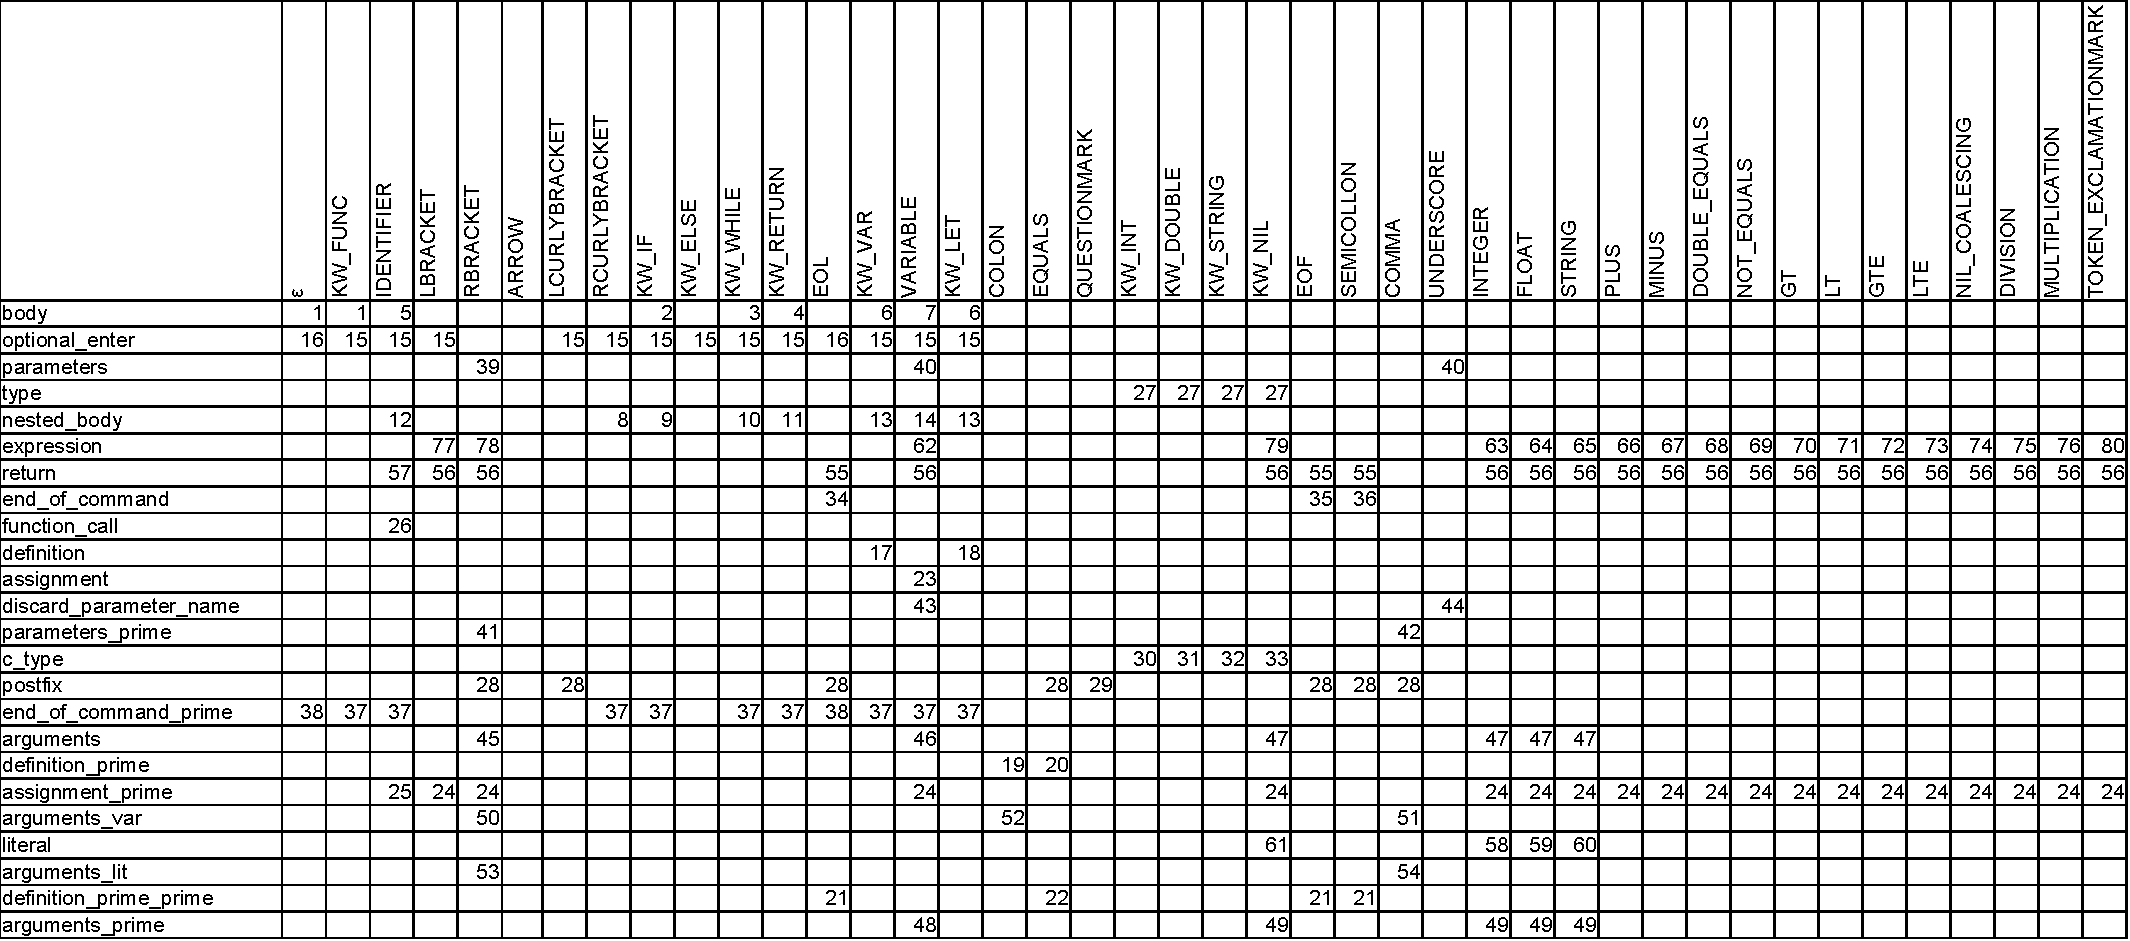
\includegraphics[scale=0.7]{LLtable.pdf}
	\caption{LL(1) table used in syntactic anlysis.}
	\label{fig:lltable}
\end{figure}


\vfill
\end{landscape}

\restoregeometry






\section{Syntactic analysis - bottom up}

When the top-down analysis detects a expression nonterminal, \texttt{parse\_expression} is called. The operator precedence parser stack is represented using \texttt{expr\_stack} which holds the individual items, \texttt{expr\_item}. Each \texttt{expr\_item} may represent either a dollar symbol, terminal or a nonterminal.

The following algorithm is implemented based on \cite[p.~236]{aho86}, first a dollar symbol is pushed on the stack, following that the \texttt{next\_token} macro is called and based on the precedence table indexed with the top terminal on the stack and the currently processed token. The table consists of the following symbols :
\begin{itemize}
\item \texttt{=} $\rightarrow$ Push the token onto the stack and read the next token.
\item \texttt{<} $\rightarrow$  Set a breakpoint on the topmost terminal on the stack and push the token onto the stack and read the next token.
\item \texttt{>} $\rightarrow$  Reduce operation.
\item \texttt{i} $\rightarrow$  Edge case for solving expression ending with variable and next line starting with an assignment.
\item \texttt{f} $\rightarrow$  Edge case when there is a dollar in the input and top of stack.
\item \texttt{\textbackslash 0} $\rightarrow$  Error case.
\end{itemize}

If a \textbf{i} symbol is obtained, we got two identifiers after each other which would usually result in an error, how ever we may have the case where the expression ends with an identifier and the next command is an assignment, so we try to finish parsing the expression just using reductions and ignoring the second identifier. If this is successful, the expression is valid and the top-down analysis continues with the second identifier, otherwise an error is raised.
When a \textbf{f} symbol is obtained, the expression is valid and the analyzer returns.

\subsection{Precedence table}

\begin{figure}[h]
	\centering
	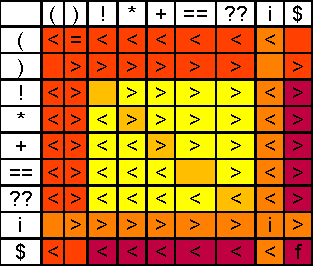
\includegraphics[scale=1.3]{Precedencna Tabulka.pdf}
	\caption{Precedence table used in syntactic analysis.}
	\label{fig:prectable}
\end{figure}



\section{Symbol table}

The symbol table was implemented according to the requirements of the task, stating the need to use a height balanced binary search tree. A splay tree was chosen to store the data, because provides advantages over general self-balancing binary search trees when accessing recently accessed items which is useful as variables are often accessed many times in succession such as during assignment and provides a time complexity of $\mathcal{O}(\log{}n)$ amortized time.\cite{Pfaff_2004}

The symbol table stores information about symbols as a structure with a type and a union of a variable and function structure as described in figure \ref{fig:symboldata} on page \pageref{fig:symboldata}.


\begin{figure}[h]
	\centering
	\includesvg{symbol_data}
	\caption{Diagram of SymbolData stored in symbol table.}
	\label{fig:symboldata}
\end{figure}

The symbol table simulates the frame stack by implementing a stack of BSTs where the bottom most frame on the stack represents the global frame and subsequent frames represent local frames. A custom lookup function is implemented to solve visibility outside of frames. The symbol table holds all the functions in a separate BST which is always accessible.


\section{Semantic analysis}
Semantic analysis ensures the logical coherence and adherence to language rules before code generation. At each variable definition, we check if the variable isn't being redefined in the current scope, this would result in a semantic error. Similar checks are run when functions are defined, we check the table for already existing user-defined functions and also built-in functions, since function redefinition is not allowed, this results in a semantic error. 

Semantic analysis also handles scoping, each time a variable is accessed, multiple checks are run to ensure the variable is defined, is accessible while \emph{variable shadowing}\footnote{Variable shadowing occurs when a local variable within a specific scope has the same name as a variable in an outer scope, leading to the inner variable "shadowing" or taking precedence over the outer one.} is properly handled.

Function signatures are another aspect that has to be checked, when a function is called, it is looked up in the symbol table, assuming it is retrieved, first the number or parameters and arguments is checked, following that their types are checked. If a function was not yet declared, it is added to the symbol table upon being called and is marked as undefined, when defined, the signature is checked. At the end of compilation, the symbol table is checked for called but undefined functions.

Finally if types are successfully inferred, each operation in the bottom-up parser checks the types, possibly implicitly converting them during expression parsing. When the expression parsing finishes a return type is generated from the last \texttt{expr\_item} on the stack used for future checks and type inference.

\section{Code generation}

Code generation is handled mostly by actions, which are called intermittently during syntactic analysis. Actions may leverage functions from the \texttt{generator.c} file. Examples of such functions are \texttt{defineVariable(char* name)} which generate code for defining inside the current scope. Scopes are handled as following, each scope has two identifiers, a \emph{recursion level} and \emph{block number}, each recursion level corresponds to a local frame in the symbol table. When a variable is generated, it is assigned the current values of \emph{recursion level} and \emph{block number} and is stored in the symbol table. When a symbol is being resolved, the symbol table first searches in the current frame corresponding to the current \emph{recursion level}, if the symbol if found, it's \emph{block number} has to match the current one, if the symbol was not found at the current \emph{recursion level}, the search continues on previous level without the need to check the \emph{block number}. Thus all variables are defined on the global frame in the interpreter and their scoping is handled by their identifiers which can be seen on page \pageref{Code example} in listing \ref{Output code}.



\newpage
 The variable \texttt{i} on line $1$ in the input code listing correctly corresponds to \texttt{i\_0\_0} in the output code on line $5$, while line $3$ of the input code also correctly corresponds to the global variable from inside the scope of the while loop on line $12$ and $15$. How ever since the line $4$ in the input code defines a new variable shadowing the previous one, the output code assigns the sum of the global \texttt{i} (line $16$) and the integer literal $1$ to the newly declared variable \texttt{i\_1\_1} on line $19$. Now that \texttt{i\_1\_1} shadows \texttt{i\_0\_0}, it is used instead on line $23$ for the \texttt{write} function.
 
Another issue was the redefinition of variables in while loops, to alleviate this problem, \texttt{defineVariable} first writes all definitions to a buffer, which is printed at the end of compilation and the interpreted code flow begins by jumping and defining all variables and returning to the main scope where flow continues as normal.

Finally code generation of expressions is handled using the above described scope resolution and stack operations.



\noindent\begin{minipage}{.45\textwidth}
\label{Code example}
\begin{lstlisting}[style=PseudoStyle, caption=Input code,frame=tlrb, label={Input code}]{Input code}
var i = 0;
while(i == 0){
    i = i + 1
    let i = i + 1
    write(i)
}

\end{lstlisting}
\end{minipage}\hfill
\begin{minipage}{.45\textwidth}
\begin{lstlisting}[style=PseudoStyle, caption=Generated code,frame=tlrb, label={Output code}]{Output code}
.IFJcode23
JUMP $$definitions
LABEL $$main
PUSHS int@0
POPS GF@i_0_0
LABEL $$while1
PUSHS GF@i_0_0
PUSHS   int@0
EQS
PUSHS bool@true
JUMPIFNEQS $$endwhile1
PUSHS GF@i_0_0
PUSHS   int@1
ADDS
POPS GF@i_0_0
PUSHS GF@i_0_0
PUSHS   int@1
ADDS
POPS GF@i_1_1
CREATEFRAME
DEFVAR TF@%retval
DEFVAR TF@%arg0
MOVE TF@%arg0 GF@i_1_1
WRITE TF@%arg0
JUMP $$while1
LABEL $$endwhile1
JUMP $$main_end
LABEL $$definitions
DEFVAR GF@i_0_0
DEFVAR GF@i_1_1
JUMP $$main
LABEL $$main_end
LABEL $$end
EXIT int@0
\end{lstlisting}
\end{minipage}




\newpage 
\part{Division of work}
In order to provide transparency and accountability, this section outlines the specific contributions of each team member to the project.
\section{Individual Contributions}

\begin{itemize}
\item Daniel Mačura - lexer, LL table and grammar, syntactic analysis (top-down and bottom-up), semantic analysis, symbol table, code generation, testing, documentation

\item Matúš Masár - lexer, testing, documentation, presentation

\item Samuel Lencsés - symbol table

\item Oliver Mokráš - 
\end{itemize}

\newpage
\bibliographystyle{enplain}
\bibliography{bib}
\end{document}